\documentclass[../psets.tex]{subfiles}

\pagestyle{main}
\renewcommand{\leftmark}{Problem Set \thesection}
\setcounter{section}{3}

\begin{document}




\section{Isotope Effects and Kinetics}
\marginnote{11/26:}The questions pertain to the material covered from Thermodynamic Isotope Effects (Nov 5) to Kinetic Rate Laws (Nov 14).
\begin{enumerate}
    \item The following schematic illustrates the six possible kinetic scenarios for the reaction
    \begin{equation*}
        \ce{\textbf{A} <=>[$k_1$][$k_{-1}$] \textbf{B} ->[$k_2$] \textbf{C}}
    \end{equation*}
    of \textbf{A} to \textbf{C} via \textbf{B}.
    \begin{center}
        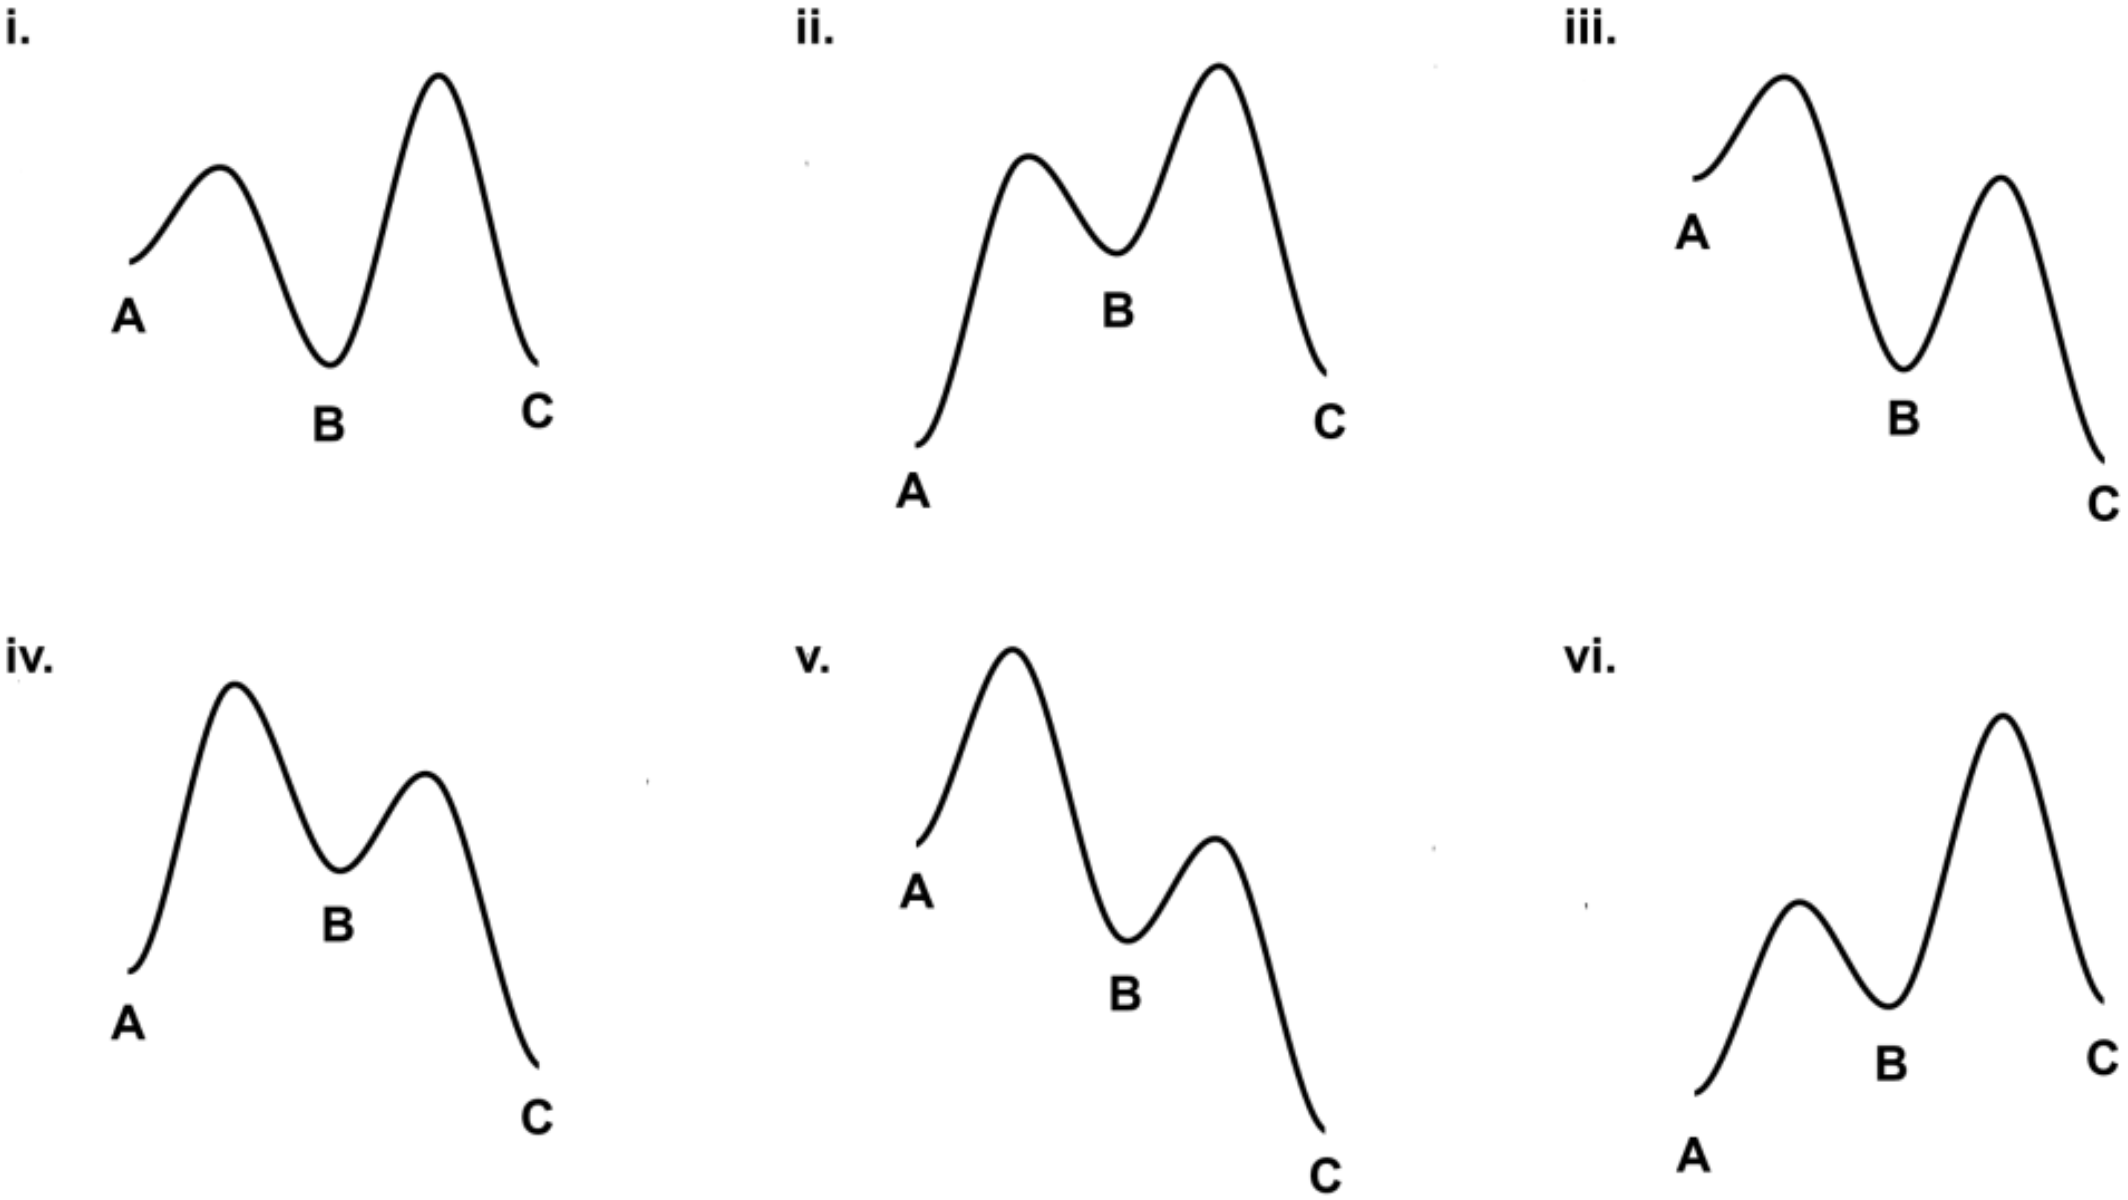
\includegraphics[width=0.7\linewidth]{PSet4F1.png}
    \end{center}
    \begin{enumerate}
        \item In which of these scenarios would the steady-state approximation \emph{not} be valid? Provide a brief explanation for your answers.
        \item In which of these scenarios would the quasi-equilibrium assumption \emph{not} be valid? Provide a brief explanation for your answers.
        \item Consider a situation where \textbf{A} is isotopically labeled. If isotopic substitution affects only the rate of conversion of \textbf{B} to \textbf{C} (and not from \textbf{A} to \textbf{B}), in which scenarios might you expect to observe an independent rate kinetic isotope effect (KIE)? Please explain.
        \item In which scenarios might you expect to observe an independent rate KIE if isotopic substitution affects only the step involving formation of \textbf{B} from \textbf{A} (and not from \textbf{B} to \textbf{C})?
    \end{enumerate}
    \pagebreak
    \item Consider the following reaction.
    \begin{center}
        \footnotesize
        \schemestart
            \chemfig{*6(-(-OMe)=-=(-(-[4]Me)(-[2]Me)-[0]\charge{135=$\oplus$}{N}(-[0])(-[:-60])-[:60]\charge{45=$\ominus$}{O})-=)}
            \arrow{->[$\Delta$]}
            \chemfig{*6(-(-OMe)=-=(-(-[:150]Me)=[:30])-=)}
            \arrow{0}[,0.1]\+{,,-2.2em}
            \chemfig{Me-[:-30]N(-[6]Me)-[:30]OH}
        \schemestop
    \end{center}
    \begin{enumerate}
        \item The mechanism for this reaction could proceed via a concerted pathway or a stepwise pathway. Provide arrow-pushing mechanisms for both processes.
        \item When the two benzylic methyl groups were deuterated, kinetic isotope effects (KIEs) of 5 and 1.2 were measured in toluene and DMF respectively. Suggest a possible explanation for the observed KIEs.
        \item When the reaction was run at two different temperatures and in two different solvents, the following rate data were obtained. Compare the activation enthalpy ($\Delta H^\ddagger$) and activation entropy ($\Delta S^\ddagger$) of the reactions in toluene and in DMF. Suggest a possible explanation for the observed differences.
        \begin{center}
            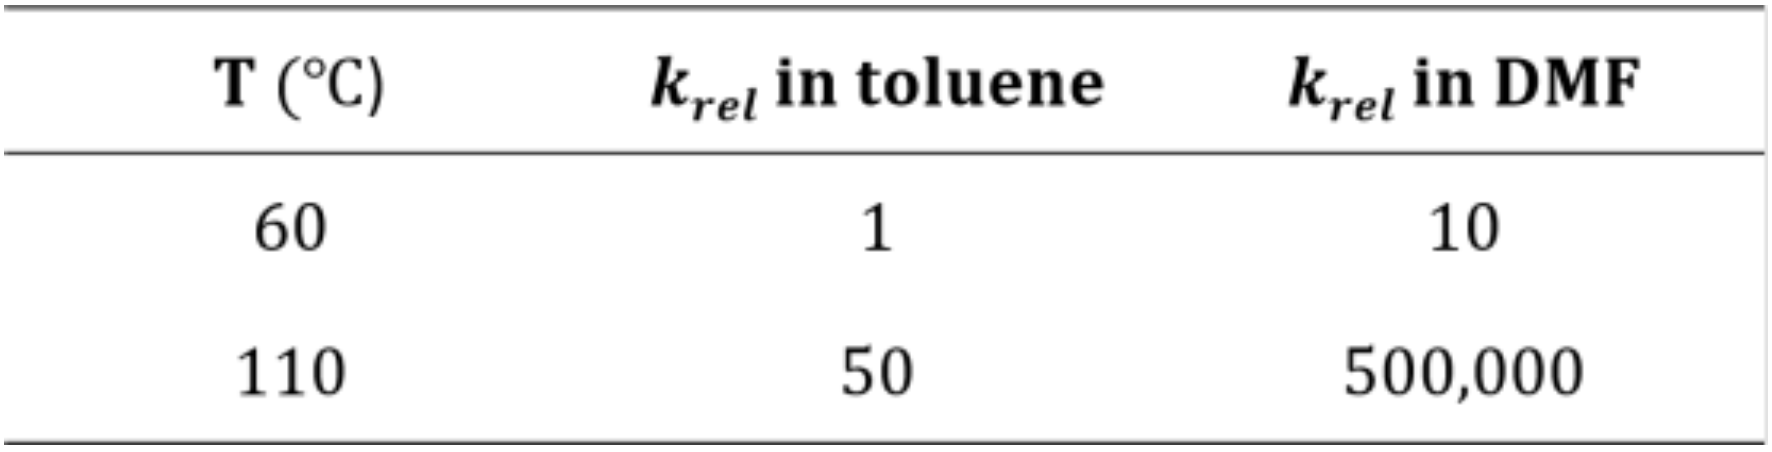
\includegraphics[width=0.4\linewidth]{PSet4F2.png}
        \end{center}
    \end{enumerate}
    \pagebreak
    \item In nonpolar solvents, compound \textbf{1} reacts thermally with \textbf{2} to give only \emph{endo} \textbf{3}.
    \begin{center}
        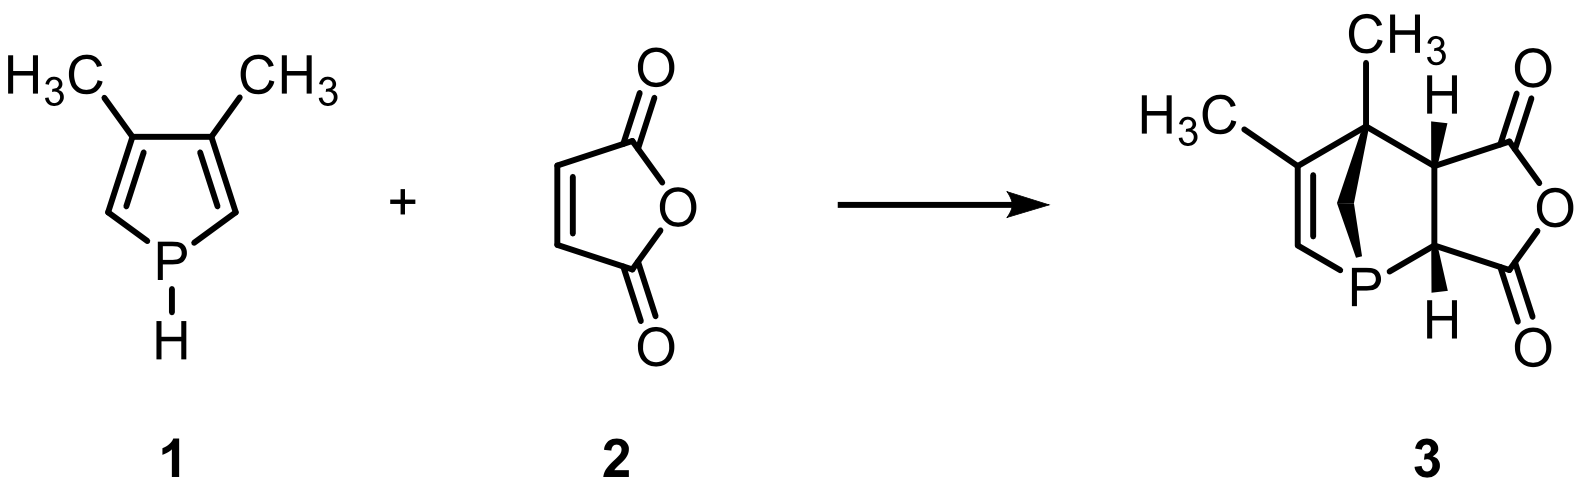
\includegraphics[width=0.55\linewidth]{PSet4F3.png}
    \end{center}
    Using small amounts of \textbf{1} and `flooding' with \textbf{2}, it has been established that the rate is pseudo-first-order in $\cnc{\textbf{1}}$. Measuring the pseudo-first-order rate constant $\kobs$ at several different concentrations of excess \textbf{2} gives a plot of the type shown below.
    \begin{center}
        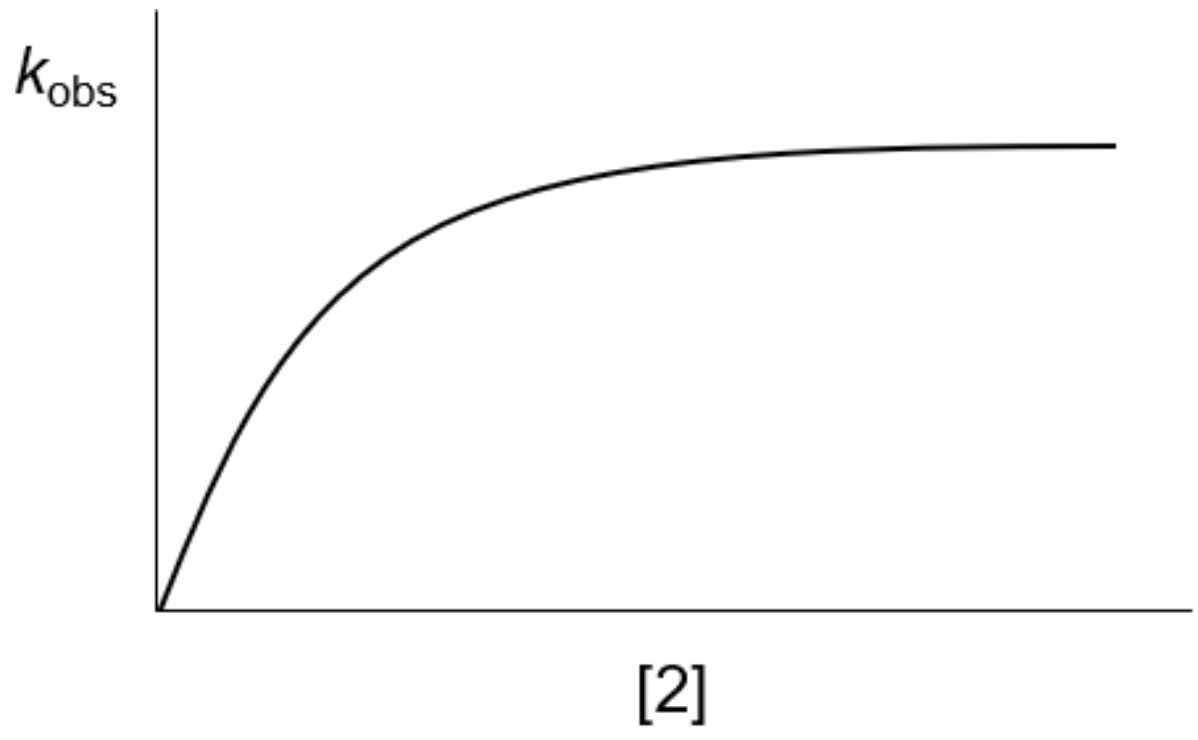
\includegraphics[width=0.35\linewidth]{PSet4F4.png}
    \end{center}
    Compound \textbf{1}, deuterated at phosphorus, undergoes exchange of \ce{D} with both $\alpha$-hydrogens, as shown below. At low concentrations of \textbf{2}, the \ce{H}/\ce{D} exchange rate is rapid compared to the rate of formation of \textbf{3}. At `saturating' concentrations of \textbf{2}, the formation of \textbf{3} occurs faster than \ce{H}/\ce{D} exchange.
    \begin{center}
        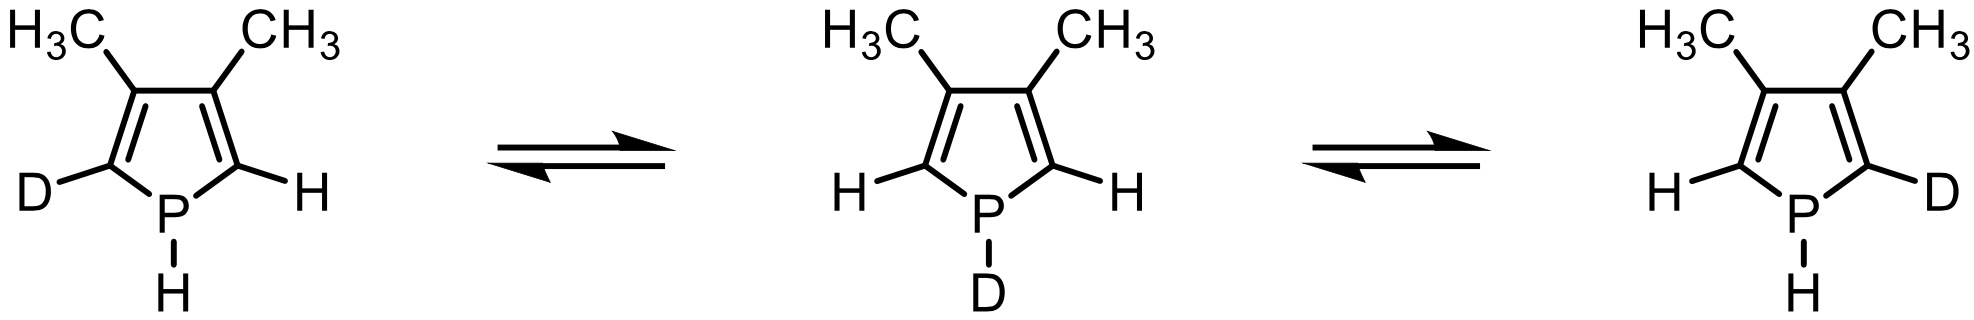
\includegraphics[width=0.7\linewidth]{PSet4F5.png}
    \end{center}
    \begin{enumerate}
        \item Write a full mechanism and a rate law for the formation of \textbf{3} that is consistent with these observations.
        \item Explain how your mechanism accounts for the labeling and kinetic behavior.
        \item Draw reaction coordinate energy diagrams at the limiting cases where $\cnc{\textbf{2}}$ is\dots
        \begin{enumerate}[label={\roman*)}]
            \item Very low;
            \item Very high.
        \end{enumerate}
    \end{enumerate}
    \pagebreak
    \item 
    \begin{enumerate}
        \item Estimate the magnitudes of the equilibrium constants ($K_1$, $K_2$) for the following reactions. Provide explanations.
        \begin{center}
            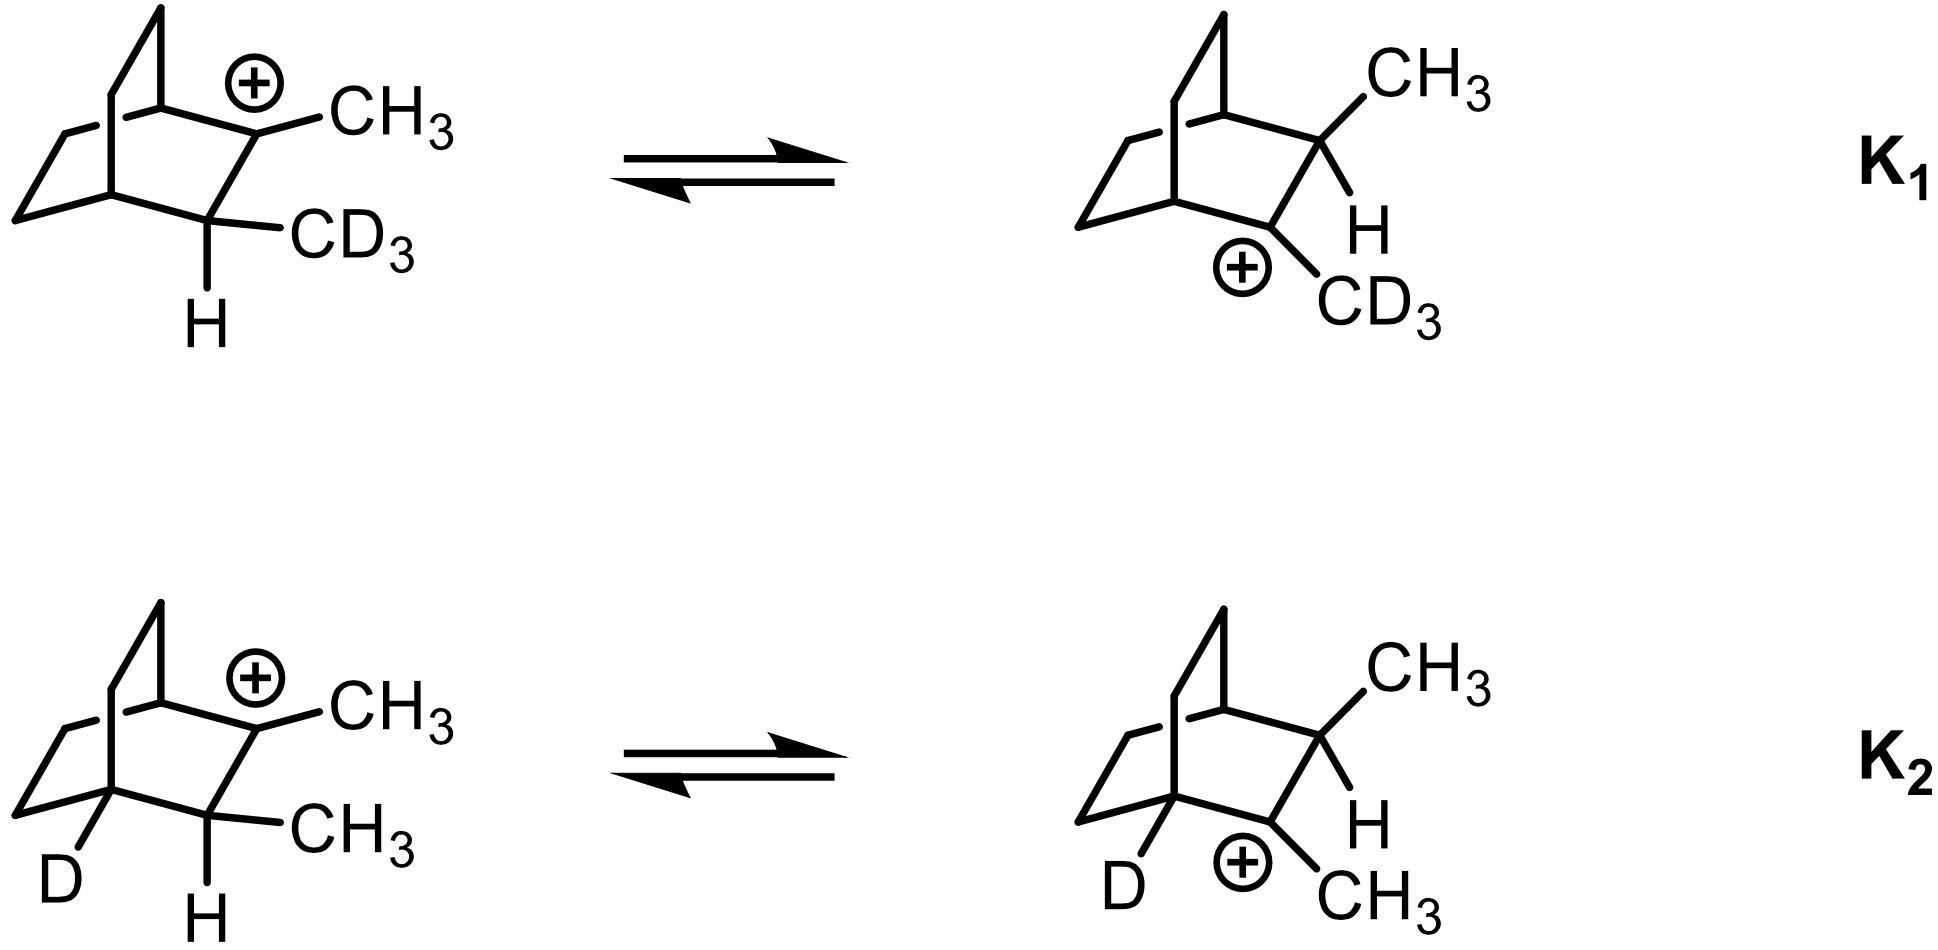
\includegraphics[width=0.5\linewidth]{PSet4F6.png}
        \end{center}
        \item Estimate the magnitudes of $\text{KIE}_1$ and $\text{KIE}_2$ for the following solvolysis reactions. Provide explanations.
        \begin{center}
            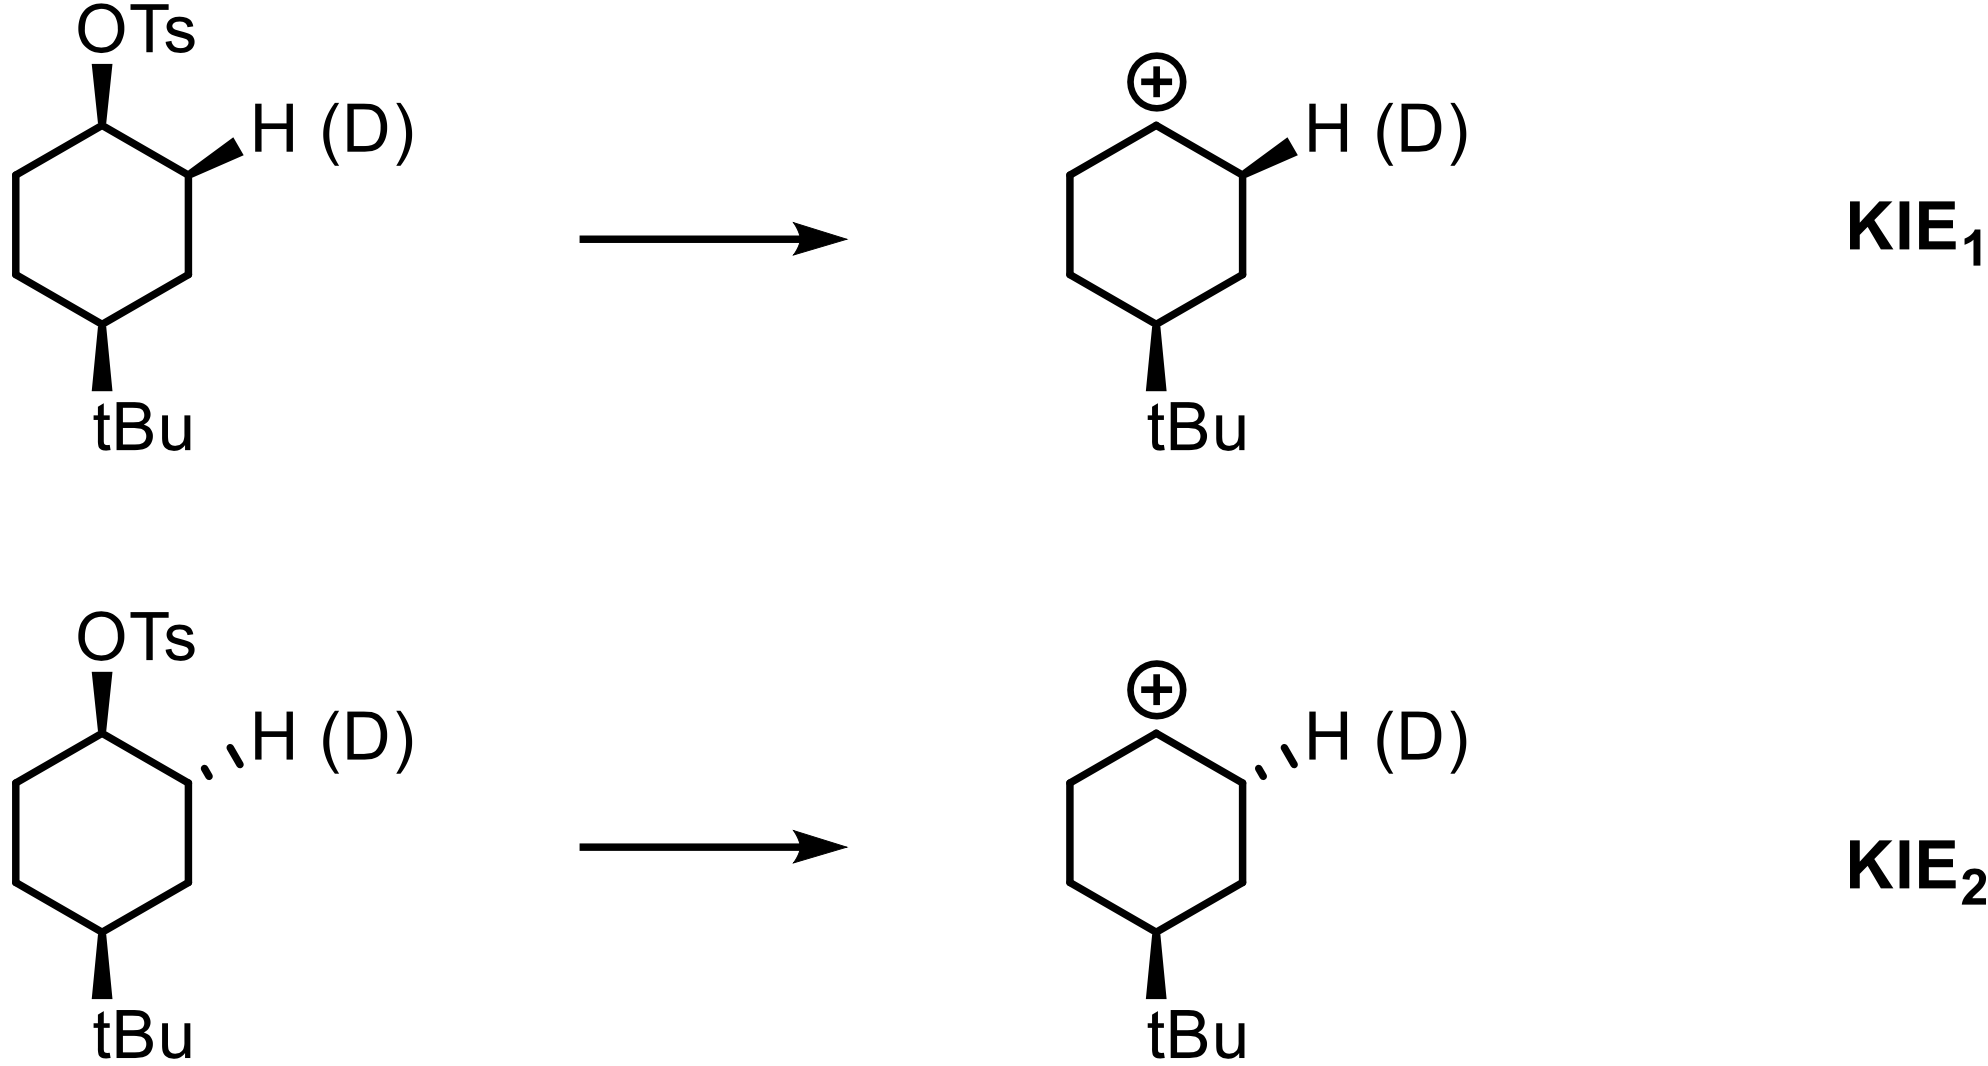
\includegraphics[width=0.55\linewidth]{PSet4F7.png}
        \end{center}
    \end{enumerate}
\end{enumerate}




\end{document}